%!TEX root = Funktionalanalysis - Vorlesung.tex
\chapter{Einf{\"u}hrung}
\section{R{\"a}ume}

Sei $X$ ein Vektorraum, $dim X < \infty $ und sei $x = (x_{1},\dotsc,x_{n})^{T} \in \MdR^{n}$
\begin{align*}
	& \|x\|_{2} := \left(\sum_{k = 1}^{n} \|x_{i}^{2}\| \right)^{\frac{1}{2}}\\
	& \|x\|_{\infty} := \smash{\displaystyle\max_{i = 1}^{n}}  \|x_{i}\|		
\end{align*}	

Diese Normen sind äquivalent, denn:
$\| x \|_{\infty} \leq \| x \|_{2} \leq n^{\frac{1}{2}} \| x \|_{\infty}$ \newline

\begin{satz}[Bolzano-Weierstra{\ss}] \index{Bolzano-Weierstrass} \label{s:1-bolzanoweierstrass}
$A \subset \MdR$ beschränkt. Dann hat jede Folge $(x_{n})_{n \in \MdN} \subset A$ eine konvergente Teilfolge.
\end{satz}

\begin{beispiel}
$X = C[0, 1] = \{ f : [0, 1] \rightarrow \MdR: f \text{ stetig auf } [0, 1] \}$
\begin{align*}
\| f \|_{2} & := \left( \int_{0}^{1} \| f(t) \|^{2} dt \right)^{\frac{1}{2}} \\
\| f \|_{\infty} & :=  \smash{\displaystyle\max_{t \in [0, 1]}}  \| f(t) \|
\end{align*}
\newline
Dabei gilt $\| f \|_{\infty} \leq \| f \|_{2}$ , aber mit folgender Funktion folgt zum Beispiel:$\hspace{0.25cm} f_n(t) = $ \\
	% todo: check this drawing / example
	\begin{figure}[H]
		\centering
		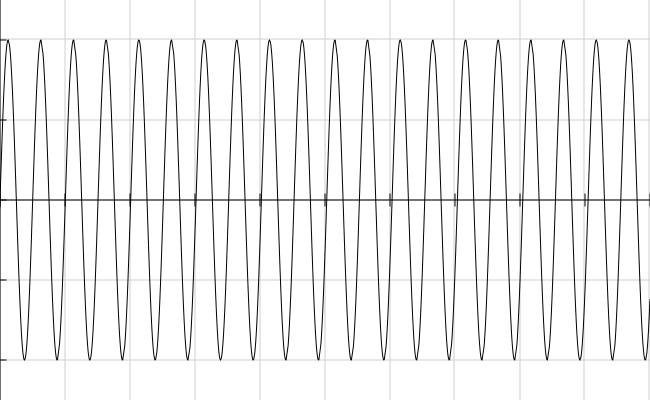
\includegraphics[width=160pt]{images/1.1.1-example1.png}
	\end{figure} \[ \text{gilt } \hspace{0.25cm} \| f_n \|_{\infty} = 1, \hspace{0.5cm} \| f_n \|_{2} \xrightarrow[n \rightarrow \infty]{} 0  
\hspace{0.5cm} \| f_{n} - f_{m} \| = 1 \text{ für } n \neq m \]
$ \Rightarrow $ \hyperref[s:1-bolzanoweierstrass]{Satz von Bolzano-Weierstra{\ss}} gilt im $\infty$-dimensionalen i.A. nicht!
\end{beispiel}

\section{Operatoren}

Sei $N = dim X, M = dim Y$ und seien $(e_n)$ bzw. $(f_n)$ Basen von $X$ bzw. $Y$. 	\\
Sei $T : X \rightarrow Y$ gegeben durch: \\
\[ \begin{xy} \xymatrix{
	X \ar[r]^T	\ar[d]_{ \alpha_{n} \rightarrow \sum \alpha_{n} e_{n} }  &   Y \ar[d]^{ \beta_{n} \rightarrow \sum \beta_{n} f_{n} }  \\
      	\MdR^{N} 	\ar[r]^A    				&   \MdR^{n}  				
} \end{xy} \]
wobei $x = \sum \alpha_{n} e_{n},\hspace{0.2cm} Tx = \sum \beta_n f_n, \hspace{0.2cm} \beta_m = \sum_{n = 1}^{N} a_{mn} \alpha_{n}. $ \\ \\
Daraus folgt:
\begin{itemize}
	\item $T$ ist stetig
	\item X = Y \gdw T injektiv \gdw T surjektiv (Dimensionsformel) \\
	(Die Gleichung $Tx = y$ ist eindeutig lösbar $\gdw$ Gleichung hat für alle $y \in Y$ eine Lösung.)
	\item Falls A selbstadjungiert ist, d.h. $A = A^{*}$, gibt es eine Basis aus Eigenvektoren $(e_{n})$ von $A$, d.h. $ T( \sum_{n=1}^{N} \alpha_{n} e_{n} ) = \sum_{n=1}^{N} \lambda_{n} \alpha_{n} e_{n}$, wobei $\lambda_{n}$ Eigenwerte sind, d.h. $A =
			\begin{pmatrix}
				\diagentry{\lambda_{1}}\\
				&\diagentry{\xddots}\\
				&&\diagentry{\lambda_{n}}\\
			\end{pmatrix} $
\end{itemize}

\begin{beispiel}
$X = C^{1}[0, 1] = \{ f : [0, 1] \rightarrow \MdR: f \text{ stetig auf } [0, 1] \}$ \\
$T f = f', T : X \rightarrow C[0, 1] \text{ stetig.} $ (Aber: $T: C[0, 1] \rightarrow C[0, 1]$, hier ist $T$ nicht definiert.) \\

$T$ ist nicht stetig bzgl. $\| \cdot \|_{\infty}$-Norm, da:
\[ f_{n}(t) = \frac{1}{\sqrt{n}}e^{int}, \hspace{0.5cm}  \text{dann: } \|f_{n}\| \rightarrow 0 \text{ für } t \rightarrow \infty \]	
\[ T f_{n}(t) = i \sqrt{n} e^{int}, \hspace{0.5cm} \text{mit: } \| T f_{n} \|_{\infty} \rightarrow \infty, \text{ für } n \rightarrow \infty \]
\end{beispiel}

\begin{beispiel}
$X = L_{2} = \{ (a_{n}): \left( \sum_{n \geq 1}^{\infty} \| a_{n} \| \right)^{\frac{1}{2}} < \infty \}$	\\
$T ( a_{1}, a_{2}, a_{3}, ...) = ( 0, a_{1}, a_{2}, a_{3}, ...)$ \\

$T$ ist injektiv, aber nicht surjektiv
\end{beispiel}

\section{Anwendungen}

\begin{enumerate}
	\item Fredholm'sche Integralglechungen \index{Fredholm'sche Integralglechung} \\
	$X = C[0, 1], \hspace{0.25cm} k: [0, 1] \times [0, 1] \rightarrow \MdR$ stetig \\
	\[ Tf(t) = \int_{0}^{1} k(t, s) f(s) ds \]
	Analogie zum endlich dim. ('Verallg. der Matrixmultiplikation'):  $ T(f_{j})(i) = \sum_{j = 1}^{n} a_{ij}f_{j}$ \\ \\
 	$T$ ist in diesem Fall linear und stetig und es gilt die Fredholm'sche Alternative:
	\[ \lambda \in \MdR \setminus \{0\}: (\lambda Id - T)(f) = y, \hspace{0.25cm} f,g \in C[0, 1] \]
	Dann existiert eine Lösung genau dann, wenn diese eindeutig ist. \\
	\item Dirichletproblem \index{Dirichletproblem}\\
	$\Omega \subset \MdR^n$ Gebiet, offen, beschränkt, glatter Rand. Sei $g: \partial \Omega \rightarrow \MdR$ stetig \\ 
	Gesucht ist ein $f \in C(\bar \Omega) \cap  C^(\Omega)$, so dass $\nabla f = \sum_{i = 1}^{n} \frac{\partial^{2} f}{\partial x_{i}^2} = 0$ in $\Omega$ und $f_{\big| \partial \Omega}= g$ \\ \\
	Beispiel: Durch Wärmeverteilung auf dem Rand auf die Wärmeverteilung im Inneren schlie{\ss}en. \\ \\
	Lösung: Dirichletintegral $J(u) = \int_{\Omega} (\nabla u )^{2} dx$, wobei $ u \in M = \{ v \in C^{1}(\bar \Omega) | \hspace{0.25cm} v_{\big| \partial \Omega} = g \}$ \\
	Sei $v_{0}$ das absolute Minimum von $J$, d.h. $J(v_{0}) = \inf \{ J(w): w \in M \}$ \\
	$v \in C^{1}(\bar \Omega)$ mit $v = 0$ in einer Umgebung von $\partial U$. $\epsilon \rightarrow J(u_{0} + \epsilon v)$:
	\[ \frac{d}{d\epsilon} J(u_{0} + \epsilon v) = \int_{\Omega} \frac{d}{d\epsilon} (\nabla u_{0} + \epsilon \nabla v)^{2} dx = 2 \int_{\Omega} (\nabla u_{0} + \epsilon \nabla v)(\nabla v) dx_{\big| \epsilon = 0} = 2 \int_\Omega (\nabla u_{0}) (\nabla v) dx \]
	Mit $0 \geq J(u_{0} + \epsilon v)- J(u_{0}) \geq 0: \hspace{0.25cm} \int (\nabla u_{0})(\nabla v) dx \overset{\text{P.I.}}{{=}} - \int (\nabla u_{0})v dx = 0$ \\
	\[ \Rightarrow \nabla u_{0} = 0 \text{, au{\ss}erdem } u_{0 \hspace{0.1cm} \big| \partial \Omega} = g \text{ (s.o.)} \]
	Im aAlgemeinen existiert das, da absolute Minimum $u_{0} \in J$ aber nicht. \\
	Ausweg: $X = \{ f \in L^{2}(\Omega), f' \in L^{2}(\Omega) \} \supset \{f \in C(\bar \Omega), f' \in C(\bar \Omega) \} $	\\
	In diesem Raum $X$ (Sobolevräume) gibt es ein Minimum $u_{0}$ von $J$. \\
	\item Sturm-Liouville Problem \index{Sturm-Liouville Problem} \\
	$X = C^{2}([0, 1]), Tu = (pu')' + qu$, mit $q \in C[0, 1], p \in C^{1}[0, 1]$ \\ 
	Problem: bei gegebenen $f \in C[0, 1]$ finde $u \in X$ mit $Tu = f, v(0) = 0, v'(1) = 0$ \\ \\
	$Y = \{ f \in L^{2}[0, 1], f' \in L^{2}[0, 1] \}$ Hilbertraum. \\
	Orthonormalbais $(e_{n})$ von $Y$ wäre: $\| e_{n} \|_{2} = 1, \int e_{n}(x) e_{m}(x) dx = 0$ für $m \neq m$ \\
	$f \in Y: f = \sum_{n = 1}^{\infty} \alpha_{n} e_{n}$ mit $\| f \|^2 = \sum | \alpha_{n} |^2$ \\
	Die $(e_{n})$ sind au{\ss}erdem Eigenvektoren des Operatoren $T$, d.h. $Te_{n} = \lambda_{n} e_{n}$ \\
	\[ Ty = f \Rightarrow \int Ty(x) e_{n}(x) dx = \int f(x) e_{n}(x) dx, y = \sum_{n = 1}^{\infty} \alpha_{n} e_{n} \]
	Gesucht sind die Koeffizienten $\alpha_{n}$
	\begin{align*}
		\int f(x) e_{n}(x) dx & = \sum_{m} \lambda_{m} \alpha_{m} \int T e_{n}(x) e_{m}(x) dx \\
							  & =  \lambda_{n} \alpha_{n} \int e_{n}(x) e_{n}(x) dx
	\end{align*}
	\[ \gdw \alpha_{n} = \frac{1}{\lambda_n} \int f(x) e_{n}(x) dx \]
\end{enumerate}

\newpage